\subsection{ICLab}
ICLab platform was used to conduct DNS, traceroute, TCP connect, TLS handshake and HTTP GET measurements. All except the traceroute experiments were successful.
\subsubsection{DNS} DNS resolution of each domain in our list was conducted from the Iranian VP using two resolvers: A local resolver of the VP's choice and the google resolver, 8.8.8.8 were used. A python script was then used to compare the DNS responses from a US-based VP to the results obtained from Iran.\\ 
All queries using the google resolver yielded a null response. We hypothesize the DNS packets destined to 8.8.8.8 are dropped. Some queries using the local resolver also yielded a null response even though a valid IP was obtained for the query using the US-based VP. On the flip side, a few domains in our test list got null response in the US and a valid IP in Iran. Figure \reminder x shows a comparison of DNS responses from a US VP and a Iranian VP.\\

\begin{figure}
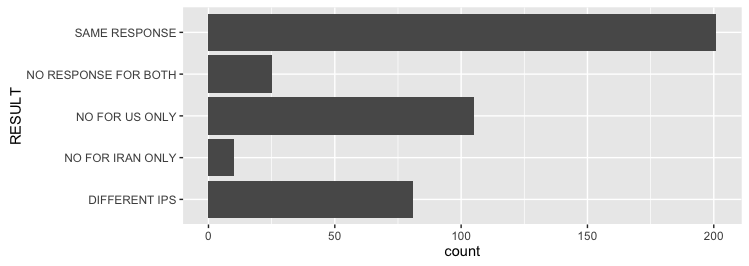
\includegraphics[
  height=.5\columnwidth,
  width=.9\columnwidth
]{pictures/DNSComparision.png}
  \caption{This is a teaser}
  \label{fig:DNSCompare}
\end{figure}

\subsubsection{Traceroute} We setup our experiment to conduct traceroute measurements before we handed it over to the person responsible for ICLab. Our intention was to pinpoint the location of the censor within Iran’s network by using the traceroute emasurements. However, we got "traceroute not found or not installed" error for all of our measurements. We see this as one of the limitations of the ICLab platform compared to RIPE atlas. Researchers do not control the remote machines in the test countries so they lack a clear expectations of what kinds of tests will be successful. \\
\subsubsection{TCP connect} 
\subsubsection{TLS handshake}
\subsubsection{HTTP}
 HTTP GET requests were executed from VPs  in both the United States and Iran to use as control and experiment results, respectively. The same test list of more than 500 urls was used. ICLab separates an url into host and path using a python library, \textit{urllib}. HTTP GET requests to invalid domains were used to verify Deep Packet Inspection(DPI). For this, paths to Alexa top websites in Iran were modified with a trigger word such as porn. The expectation is that an invalid domain should return a 404 Page Not Found Error.\\
HTTP GET requests gave a more representative view of censorship in Iran. Many domains with successful TCP handshake gave 4xx responses. We believe that  the TCP connect succeeds because the collateral damage of IP-based blocking has deterred Iran from conducting IP-based blocking. While mix of status codes 200, 400, 3xx, 403 and 404 were obtained from the Iranian VP, the same test list of URLs resulted in a negligible number of failures when run from a U.S-based VP.  A handful of error responses gotten for the US VP were usually  404 Page Not Found or 403 Forbidden. 404 error occurred in the case where the domain name was intentionally invalid like in the case of path modification to check for deep packet inspection. Some websites such as http://ladysun.net -a Women's rights website, http://www.alrased.net/site- a minority faith website, http://www.jawanan.org and http://www.jebhemelli.org- two political reform websites and a few other websites elicited a 403 response even from the US based VP. A traceroure measurement and geoIP lookup located the destination servers to be in countries such as  Japan and the U.S.  The reason for this censorship is unknown to us and would be a good thing to look at in future studies.\\
We were also able to verify the use of DPI by iran. An invalid domain should return a 404 Page Not Found Error, however, the invalid domains which had a trigger word in the path resulted in 403 Forbidden. Adding /porn to a path always resulted in a 403 Forbidden response from Iranian VP and 404 Not Found response from a U.S-based VP. \\ 



